\section{Thermoelastic stress analysis in homogeneous material (3~D)}
\subsection{Definition}
The top and the bottom of a solid body that consists of one homogeneous  material are heated. The aim of the calculation is to find out the isotropic state of stress that is reached after the whole solid is heated. 
%
Figure \ref{fig61} shows a sketch of the calculation area assuming a homogeneous solid, a constant temperature in the whole body at the beginning and a heating of the top and the bottom of the body about 10~K.
Linear elastic material behaviour, isotropic thermal expansion and no gravity effect are assumed.
%
The $xy$-plane is the horizontal plane. The height of the body is in $z$-direction. The dimensions of this 3~D-model are 10~m in all directions. 
As deformations in $x$- and $y$-direction are suppressed, the increasing temperature evokes stresses within the solid. 
The used parameters of the solid represent the material behaviour of concrete (Table \ref{tab61}).

\begin{figure}[htbp]
\centering
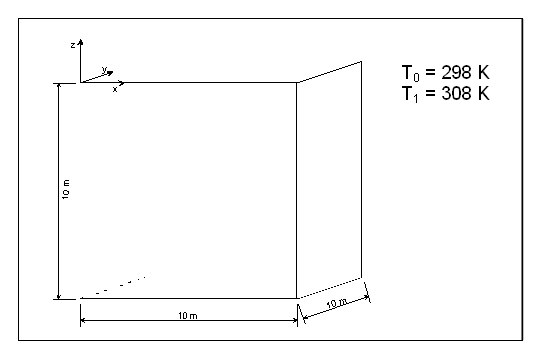
\includegraphics[width=0.6\textwidth]{PART_III/TM/figures/fig61}
\caption{Calculation area with one material}
\label{fig61}
\end{figure}

\begin{table}[htbp]
\centering
\caption{Model parameters}
\label{tab61}
\begin{tabular}{llrr}
\toprule
Symbol & Parameter & Value & Unit \\
\midrule
$T_0$  & Initial temperature (before heating) & 298 & $K$ \\
$T_1$  & Temperature after heating & 308 & $K$ \\
$\rho$  & Density of the solid &  2200 & $kg \cdot m^{-3}$  \\			
$E$ & Young's modulus of the solid & 25 & $GPa$ \\
$\nu$ & Poisson ratio & 0.27 & $-$ \\
$\alpha$ & Linear thermal expansion & 6.0$\cdot$10$^{-6}$ & $K^{-1}$ \\
$c$      & Specific heat capacity & 1.0 & $J\cdot kg^{-1}\cdot K^{-1}$ \\
$\lambda$ & Thermal conductivity & 1.0 & $W\cdot m^{-1}\cdot K^{-1}$ \\
\bottomrule
\end{tabular}
\end{table}


\subsection{Solution}
\subsubsection{Analytical solution}
The analytical solution can be derived from the time independent equation \eqref{eq61} to \eqref{eq63} with the assumptions of no deformation and an isotropic thermal expansion:
\begin{eqnarray}
\varepsilon_i & \equiv & 0 \nonumber \\[1.5ex]
\sigma_x & = & \sigma_y\,=\,\sigma_z\,=\,
-\frac{\alpha\cdot\Delta T\cdot E}{1-2\cdot\nu}
\label{eq64}
\end{eqnarray}
Equation \eqref{eq64} provides the stresses after heating the solid and shows an isotropic state of stress.

\subsubsection{Numerical solution}
The dimensions of this 3~D-model are 10~m in all directions. Deformations perpendicular to the outer surfaces are suppressed. The initial temperature in the whole area is 298~K. At the top and at the bottom of the model thermal boundary conditions are set with a temperature of 308~K. Thereby the heating of the solid about 10~K is simulated. 1000 hexahedral elements and 1331 nodes are used. The calculation is divided in 384 time steps with a constant time step length of 900 seconds. That means the heating of the solid within 4 days is simulated. The calculation model is sketched in Figure \ref{fig62}.


\begin{figure}[htbp]
\centering
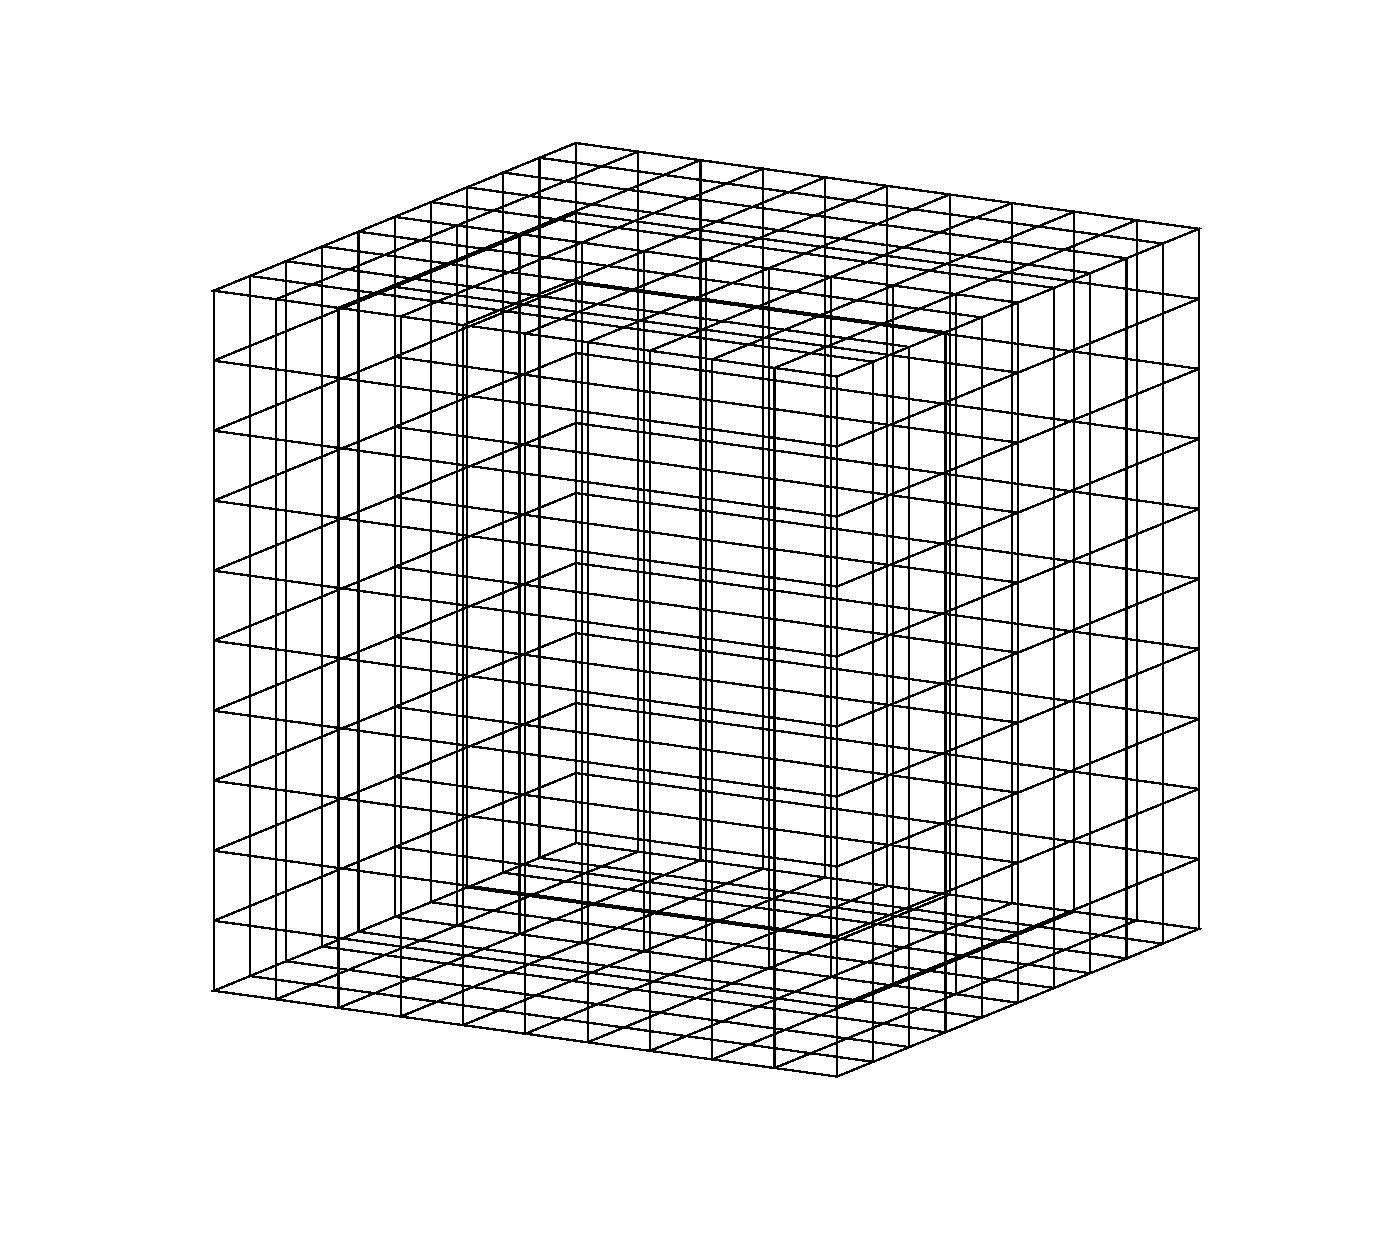
\includegraphics[width=0.6\textwidth]{PART_III/TM/figures/fig62}
\caption{Mesh for TM coupling homogeneous material 3D model}
\label{fig62}
\end{figure}

\subsection{Results}
With the analytical solution in equation \eqref{eq64} and the used parameters the stress values in the solid amount. This isotropic state of stress is reached after the whole solid is heated. The temporal development of the stresses in the centre of the model (at node 665) calculated is presented in Figure \ref{fig63}. The results of the 3~D simulation show an exact agreement with the analytical solutions.

\begin{figure}[htbp]
\centering
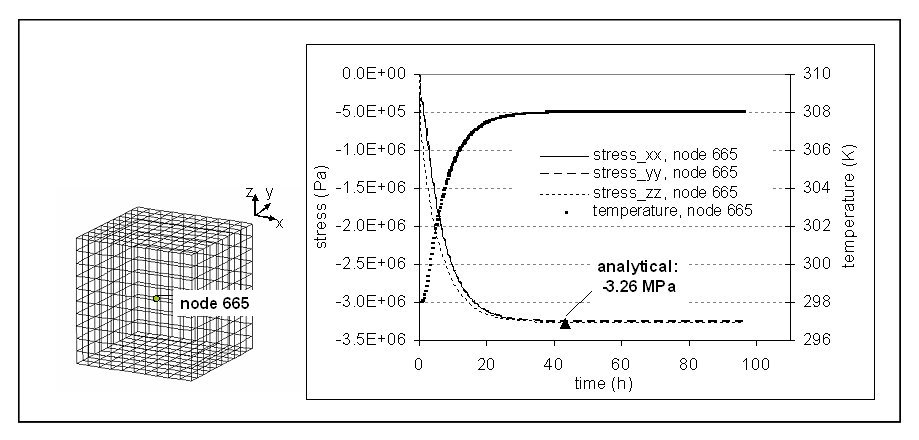
\includegraphics[width=0.9\textwidth]{PART_III/TM/figures/fig63}
\caption{Temporal stress development in the centre of the calculation model (node 665)}
\label{fig63}
\end{figure}

